\documentclass[10pt, final]{article}
%\usepackage[document]{ragged2e}
\usepackage[utf8]{inputenc}

\usepackage{fancyhdr}
\setlength{\headheight}{15pt}
 
%\pagestyle{fancy}
%\fancyhf{}
%\rhead{Uganda Pollution - Grid Summary}
\cfoot{\thepage}

\maxdeadcycles=200

\usepackage{multirow}
\usepackage{siunitx}
\usepackage{booktabs}
\usepackage{hyperref}

\usepackage{soul}
\usepackage{caption}

\usepackage{enumerate}
\usepackage{amssymb}
\usepackage{amsmath, mathtools}
\usepackage{amsopn}
\usepackage{amsthm}
\usepackage{color}
\usepackage{xcolor}
\usepackage{amsfonts}
\usepackage[makeroom]{cancel}
% \usepackage{wasysym}
\usepackage[paperwidth=8.5in,left=1in,right=1in,paperheight=11.0in,top=1in, bottom=0.5in]{geometry}

\usepackage{tikz}
\usetikzlibrary{decorations.markings}

\usepackage{pgfplots}

\pgfplotsset{compat = 1.15}
%\pgfplotsset{scaled y ticks=false}
\usetikzlibrary{positioning}
\usepackage{mathtools}

\usepackage{listings}

\DeclarePairedDelimiter\ceil{\lceil}{\rceil}
\DeclarePairedDelimiter\floor{\lfloor}{\rfloor}

\DeclareMathOperator{\im}{im}
\DeclareMathOperator{\detr}{det}
\DeclareMathOperator{\var}{var}
\DeclareMathOperator{\cov}{cov}
\DeclareMathOperator{\Real}{Re}
\DeclareMathOperator{\sgn}{sgn}
\DeclareMathOperator{\argmax}{argmax}
\DeclareMathOperator{\vect}{vec}


% Additional commands/shortcuts to make our life easier
\newcommand{\bm}{\begin{bmatrix}}
\newcommand{\fm}{\end{bmatrix}}
\def\a{\alpha}
\def\b{\beta}
\def\g{\gamma}
\def\D{\Delta}
\def\d{\delta}
\def\z{\zeta}
\def\k{\kappa}
\def\l{\lambda}
\def\n{\nu}
\def\e{\varepsilon}
\def\r{\rho}
\def\s{\sigma}
\def\S{\Sigma}
\def\t{\tau}
\def\x{\xi}
\def\w{\omega}
\def\W{\Omega}
\def\th{\theta}
\def\p{\phi}
\def\P{\Phi}
\newcommand{\pa}{\mathcal \partial}
\newcommand{\No}{\mathcal N}

\usepackage{lscape}

\usepackage{graphicx}
\graphicspath{ {./Regression_Graphs/} }

\newcommand{\hatxi}{\hat{\mathbf{x}}^i}
\newcommand{\tildexi}{\tilde{\mathbf{x}}^i}


\title{Trade - Assignment 2}
\author{Jeanne Sorin}
\date{\today}

\begin{document}

\maketitle

\input{"Table1.tex"}
The table above shows the results for the regression of log (non-zero) trade flows on log bilateral distance, a contiguity indicator, a common-language indicator, exporter-year FE, importer-year FE for the years 2000-2006. \\
We can see that the point estimates and standard errors are numerically identical across the different estimators, as they should be. Indeed, we are estimating the same model, with the same data! We are simply trying to exploit different numerical "shortcuts". If one looks carefully, we see that the estimates and standard errors differ slightly across columns. I believe this is due to numerical approximation.
\\
The number of observations are the same for the first 3 columns, but different for the 4th column. My understanding is the observations dropped in the last columns are \textit{"singleton"} observations, i.e. corresponding to pairs of FE \textit{exporter-year + importer-year} containing a single observation. Therefore, no variation remains to explain once we control jointly for the 2 pairs of FE.
\\
THe R2 in column 2 is different than in column 2 because of the panel structure we impose by using \textit{xtreg}: the R2 reported with panel data models is cross-sectional rather than also across time (as for the 3 other columns).
\\
Finally, we notice that the relative computation times of these estimators depend on the "\textit{net}" dimensionality and size of the data. To be more precise, we see that \textit{reg}, which takes the \textit{raw} data is obnoxiously slow, while \textit{reghdfe}, which "nets" out both pairs of FE before performing the regression, is much faster, as the net dimensionality is exponentially smaller. The speed doesn't seem to depend on the number of observations.

\newpage
\begin{landscape}
\center
\input{"Table2.tex"}
\end{landscape}
Regarding whether the results are sensitive to the inclusion of $0$, the answer is "\textit{it depends}". Indeed the log-linear model gives dignificantly different results between columns 2 and 3. This is unsurprising: by excluding the zero trade flows observations, we actually estimate a different (conditional) model.
Therefore, we see here that estimating a gravity equation through OLS and log is problematic because it de facto gets rid of observations with 0 trade flow.
\\
However, when one estimates the constant-elasticity specification by running the \textit{"ppmlhdfe"} command to implement the PPML estimator (columns 7 and 8), we see that estimates are really close to each other. ppml doesn't seem to suffer from the same flawn as the OLS approach to estimate gravity equations.
\\
Regarding the impact of making the dependent variable $log(x+1)$, the answer is that it performs quite poorl for the log-linear regression (columns 1 vs 2), i.e. we get quite different results. If ever one found that the results displayed in table 2 were not that different (see for example the coefficient for \textit{log distance} in column 3), one should try to run the same regression with $log(x+0.1)$ or any arbitrarily small number and would see that estimates are really off.
\\
Results from the log-linear regression are quite heteroskedastic: running a Breusch-Pagan test in stata on the model corresponding to Table 2, Col 1, we find that $chi2 = 181.32$ and $Prob > chi2 = 0.0000$. Since the latter is $< 0.05$, we can reject the null hypothesis and we conclude that there is heteroskedasticity in the data.
\\
Moreover, as one can see on the scatter plot below, the residuals' variance decreases with the fitted value, suggesting that the error does not have constant variance, i.e. that we are in the case of heteroskedasticity.
\begin{figure}[h!]
\center
	\caption{Illustrating Heteroskedasticity}
	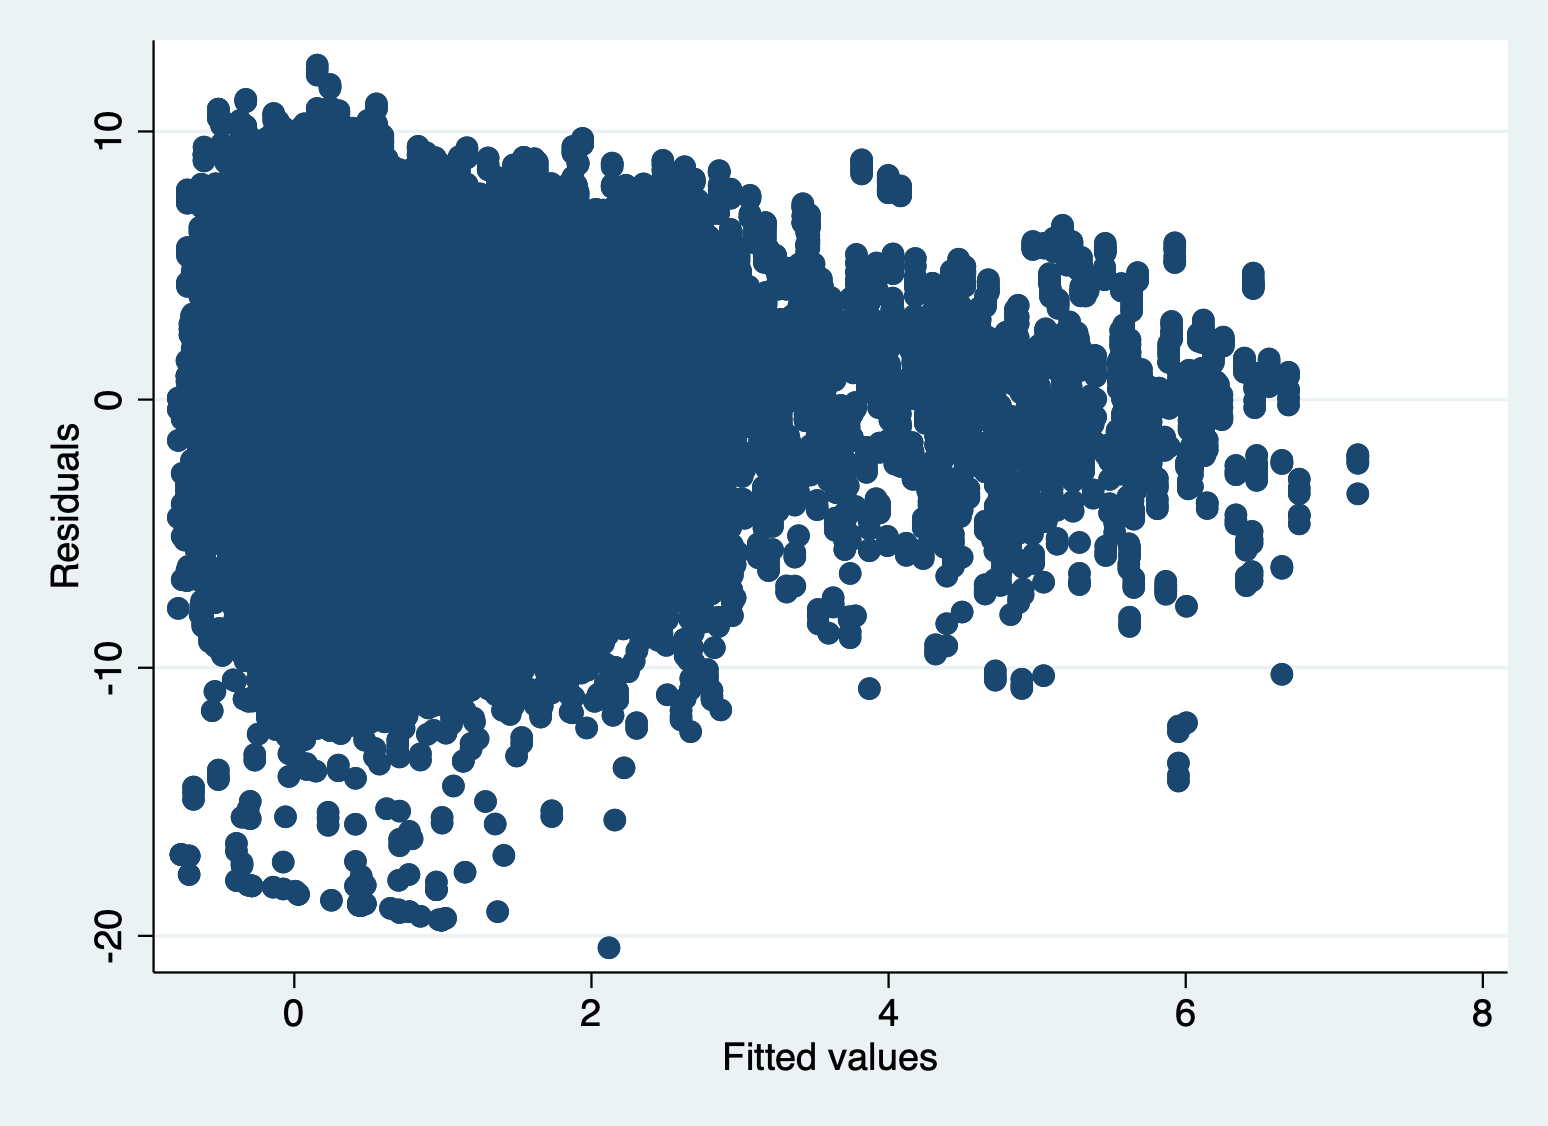
\includegraphics[width=10cm]{stata_table2_scatter.png}
\end{figure}
Finally, with respect to computation times, well, in a nutshell: the OLS approach can be really fast when using \textit{reghdfe}, but is problematic because it doesn't deal with the zeros (no free lunch I guess). On the other hand, the ppml approach is slower, but is able to deal with zeros. While \textit{ppml} is the turtle of the race, \textit{ppmlhdfe} does quite well (and is not sensitive to including the zeros or not!). \textit{poihdfe} is very decent.



\newpage
\begin{table}[htbp]\centering
\def\sym#1{\ifmmode^{#1}\else\(^{#1}\)\fi}
\caption{Table 3 }
\begin{tabular}{l*{1}{c}{c}{c}}
\hline\hline
                    &\multicolumn{1}{c}{(1)} & \multicolumn{1}{c}{(2)} & \multicolumn{1}{c}{(3)}\\
                    &\multicolumn{1}{c}{log(flow)} &\multicolumn{1}{c}{log(flow)} &\multicolumn{1}{c}{log(flow)}\\
\hline
Contiguous countries (dummy)&       0.550\sym{***} 	& 0.5495$^{***}$ & 0.550*** \\
                    &    (0.0160)        &(0.0160) & (0.016) \\
[1em]
Common language (dummy)&       0.762\sym{***} & 0.7620$^{***}$ & 0.762***\\
                    &   (0.00774)        & (0.0077) &(0.008) \\
[1em]
Log(distance)       &      -1.325\sym{***} & -1.325$^{***}$ & -1.325***\\
                    &   (0.00379)	&(0.0038) & (0.004)\\
\hline
N                   &      709,248        & 709,573  & 709,248\\
R2                  &       0.702        & 0.70258  & 0.702\\
Time (sec)          &       7.789         & 0.66837 & 2.43\\
Software 			& 		Stata		& 	R  & Julia\\
\hline\hline
\multicolumn{2}{l}{\footnotesize Robust Standard errors in parentheses}\\
\multicolumn{2}{l}{\footnotesize \sym{*} \(p<0.10\), \sym{**} \(p<0.05\), \sym{***} \(p<0.01\)}\\
\end{tabular}
\end{table}

As one can see on the table above, the three packages return the same estimates. The standard errors are also equal, up to numerical approximation.
\\
Well, R is faster, and by an order of magnitude at least!



% section problem_5 (end)



\end{document}
